\documentclass[letter,11pt,oneside]{article}
% /home/wayne/iraf/smtsci/doc/ParallacticAngle.tex
%%% (occur "\\(\\\\[a-z]*section\\|appendix\\|input\\|\\<include\\>\\)")

%%\documentclass[11pt,twocolumn]{article}
%%\usepackage[inline]{asymptote}   %% Inline asymptote diagrams
%%\usepackage{wglatex}             %% Use this one and kill others.
\usepackage{color}               %% colored letters {\color{red}{{text}}
\usepackage{fancyhdr}            %% headers/footers
%%\usepackage{fancyvrb}            %% headers/footers
\usepackage{datetime}            %% pick up tex date time 
\usepackage{lastpage}            %% support page of ...lastpage
\usepackage{times}               %% native times roman fonts
\usepackage{textcomp}            %% trademark
\usepackage{amssymb,amsmath}     %% greek alphabet
\usepackage{parskip}             %% blank lines between paragraphs, no indent
\usepackage{shortvrb}            %% short verb use for tables
\usepackage{lscape}              %% landscape for tables.
\usepackage{longtable}           %% permit tables to span pages wg-longtable
\usepackage{url}                 %% Make URLs uniform and links in PDFs
\usepackage{enumerate}           %% Allow letters/decorations for enumerations
\usepackage{endnotes}            %% Enhance footnotes/endnotes
\usepackage{listings}            %% Make URLs uniform and links in PDFs
\pdfadjustspacing=1                %% force LaTeX-like character spacing
\usepackage{geometry}            %% allow margins to be relaxed
%%\usepackage{wrapfig}             %% permit wrapping figures.
%%\usepackage{subfigure}              %% images side by side.
\geometry{margin=1in}            %% Allow narrower margins etc.
\usepackage[T1]{fontenc}         %% Better Verbatim Font.
\renewcommand*\ttdefault{txtt}   %% 
%%\usepackage{natbib}   %% bibitems
\usepackage[bookmarks]{hyperref} %% Make huperlinks within a PDF

%% include background image (wg-document-page-background) 

\usepackage{graphicx}            %% Include pictures into a document
%% (wg-texdoc-inserttikz)


\def\documentisdraft{DRAFT}
\def\documentreview{NOTREVIEW}

%% (wg-texdoc-isdraft)


\def\reviewtest{REVIEW}
\def\drafttest{DRAFT}
\def\wgdocdate{27 Mar, 2019}
\def\wgdocdatetime{\wgdocdate~ at \currenttime}
\ifx\documentisdraft\drafttest
\usepackage[left]{lineno}   %%%%%%%%%%%%% DRAFT
\usepackage{draftwatermark}
\SetWatermarkScale{5.0}
\SetWatermarkColor[gray]{0.3}
\fi

%% (wg-texdoc-insert-fancy-headers)


%% Uncomment for DSES style header/footers
\pagestyle{fancy}
\lhead{Paralactic Angle \wgdocdate}
\rhead{UNDER DRAFT\\Page \thepage~of \pageref{LastPage}}
\lfoot{Created 27Mar2019}
\rfoot{Version 0.1 UNDER DRAFT}
\ifx\documentisdraft\drafttest
\cfoot{Draft \wgdocdatetime}
\fi
\renewcommand{\footrulewidth}{0.4pt}


%%\usepackage{makeidx}             %% Make an index uncomment following line
%%\makeindex                       %%.. yeah this one, too. index{key} in text
%%

\definecolor{verbcolor}{rgb}{0.6,0,0}
\definecolor{darkgreen}{rgb}{0,0.4,0}
\newcommand\debate[1]{\textcolor{darkgreen}{DEBATE: #1} \marginpar{\textcolor{red}{DEBATE} }}
\newcommand{\ltodo}[2]{\marginpar{\textcolor{red}{ACTION: #1}\endnote{#2}}}
\renewcommand{\thefigure}{\thesection-\arabic{figure}}
\newcommand{\menu}{\ensuremath{\;\rightarrow\;}}
\newcommand{\dhl}[1]{{\color{verbcolor}{\texttt#1}}}
%%(wg-add-inline-images)  %% add inline images to the mix
\newcommand{\target}{{\color{red}{TARGET TBD~}}}
\newcommand{\then}{{\color{red}{DATE TBD~}}}
\newcommand{\guidemodel}{{\color{red}{GUIDEMODEL TBD~}}}
\newcommand{\miles}{{\color{red}{MILES STAR TBD~}}}
\newcommand{\tbd}{{\color{red}{TBD~}}}
%\newcommand{}{{\color{red}{TBD~}}}


%%Begin User Definitions: Hint: ~/.latex.defs and  latex.defs  
%%End User Definitions:
%%(wg-texdoc-adjust-paper-width)
%% (wg-texdoc-insert-hypersetup)

%%% PDF Fields uncomment \usepackage[bookmarks]{hyperref} above.
\hypersetup{
colorlinks=true,
linkcolor=red,
citecolor=red,
urlcolor=blue,
pdfauthor = {Copyright(c) 2015. All rights reserved. Wayne Green},
pdftitle = {A TeX Document},
pdfsubject = {My Subject Stuff here},
pdfkeywords = {Keyword1, Keyword2, ...},
pdfcreator = {LaTeX with hyperref package},
pdfproducer = {dvips + ps2pdf}}


%%%%%%%%%%%%%%%%%%%%%%%%%%%%%%%%%%%%%%%%%%%%%%%%%%%%%%%%%%%%%%%%%%%%%%%%%%%%%


\begin{document}


%% (wg-latex-pretty-title-page)
%% (wg-texdoc-titleblock)


\title{Parallactic Angle and Instrumentation Issues for Small Telescope Spectrography}
\author{Wayne Green \\
Forrest Sims}
\date{\wgdocdatetime}
\maketitle

\begin{abstract}
We explore the ramification of noise related to parallactic angle,
atmospheric effects, extinction, deflection, optical distortion,
focus, alignment, slit alignment, cosmic rays, processing artifacts
and sensor noise on spectra taken with small telescopes. We offer a
framework of tests and tricks  to qualify, correct and report the
impact of these sources when creating publishable data. A public set
of data is provided for training and test suites for processing
approaches.

\end{abstract}

%%%%%%%%%%%%%%%%%%%%%%%%%%%%%%%%%%%%%%%%%%%%%%%%%%%%%%%%%%%%%%%%%%%%%%%%%%%%%
%% table of contents
%%%%%%%%%%%%%%%%%%%%%%%%%%%%%%%%%%%%%%%%%%%%%%%%%%%%%%%%%%%%%%%%%%%%%%%%%%%%%
 
\pagenumbering{roman}   % i,ii,etc
%%\pagenumbering{gobble}   %ignore page numbers for a while
%%\pdfbookmark[0]{Table of Contents}{MyTOC} % if usepackage{hyperref} in use.
%%\tableofcontents
%%\listoffigures
%%\listoftables
%%\newpage


\setcounter{section}{0}
\pagenumbering{arabic}

\ifx\documentisdraft\drafttest
\linenumbers    %%%%%%%%%%%%% DRAFT
\fi

\ifx\documentreview\reviewtest
\vspace{-.15cm}
\begin{enumerate}\addtolength{\itemsep}{-0.5\baselineskip}
   \item   Your experiment of quickly rotating the spectrograph
90 degrees with the mounting screws.
   \item   deflection - subtracting cals and seeing artifacts
   \item   Fishtail optical distortion and need to cheat the blue lines
of cal line list
   \item   spe vs cosmic rays -- that time you had that one pesky pixel
and the 3D code I wrote for grins to see it
   \item   slit alignment -- still needs some test and math. This is where
the angle of the slit w.r.t. the lines of the grating. We'll see this
with the rotation of the alpy and other slits; and with the Ovio
slit in its holder w.r.t. the detent ball-bearing.
   \item   lamp alignment (alpy if the lamp is off) we're testing that now.
   \item   focus the quick check using a blended line
   \item   get the public data set together, in the SAS\_Spectroscopy
Github, and include that repository in the paper.
   \item platesolve guide image, use ds9 to look at the parallactic angle
   \item  I have to produce 2 colored graphs, subjective badness with
the slit parallel to ra vs parallel to dec.
   \item  The graph I do have that shows apparent position as function
of altitude.
   \item   A chart for various altitudes.
   \item   The algorithm for parallactic angle using vectors -- working
code needs that last minute check for brain toots.
   \item  Rotation of the slit w.r.t. the grating's dispersion lines.
\end{enumerate}
\fi

\section{Overview}

Data of \target was taken on \then using a Planewave-14 and a Shelyak
LISA spectrograph ($\sim$ R 900) using an Atik 414EX camera and a
Starlight Express \guidemodel.  During reduction of a spectrum of
\target the blue end of the spectrum appeared dim by about 50\%. It
was apparent from the data parallactic angle was to blame. The main
recommendation for amateur spectroscopy has been to have the slit
parallel to Delcination to manage tracking difficulties for
instruments without permenant mounts. 

A quick experiment was devised to test parallactic angle's impact. A
Miles reference star \miles was chosen to the north and near
transit. The instrument is mounted to the telescope backplate with 4
screws making a rapid (~15 minutes) 90 degree rotation possible with
no appreciable change in focus.  An image was taken with the slit
orientation parallel-Declination, the instrument rotated and a new
image was taken with a parallel-RA orientation. Figure \tbd shows the
result.  The use of a image rotator resulted in dramatic reduction of
parallactic angle for spectra.

This problem led to the question of where in the sky is a
parallel-Declination slit orientatin good and where is it bad? How is
the parallactic angle best computed? How is the angle expressed and
communicated to control programs?  

For completeness, the experiment was expanded to understand other
issues with small telescope spectroscopy to understand how other
influences with the instrument package require attention during
planning and operations.

During processing of the spectra, we noted mechanical deflection
(Young's modulus) within the spectrograph shifted spectra several
angstroms with respect to calibration lamp images.  Remediating the
somewhat arbitrary and cavilier approach to taking calibration lamp
images is discussed.

\ltodo{Make target figure}{Show the original problem}
\ltodo{Miles Star figure}{show the experiment}

\subsection{The Parallactic Angle}

In simple terms, the atmosphere acts like like a prism. Physics shows
atmospheric dispersion to be a function of the index of refraction of the
medium. The atmosphere is a piece-wise continusouly varying fluid
medium with a pressure gradient with distinct, sharp but continuous
boundary conditions. To what degree do the fine points of the actual
physics have to be satisfied in a parallactic angle algorithm?

\ltodo{Diagram}{Parallactic angle diagrams. Panel 1 vectors,
2 spherical triangles}

The parallactic angle is taken from north through east with its apex
at the target and terminus at the observatory. This angle is greater
than 180 degrees for targets east of the meridian.  The common
subjective solution uses simplified spherical triangles, computes the
compliment of the angle for targets to the east and actually comes
close for the case where the target is west of the meridian. The human
mind can spot this and easily make the adjustment. Computers can get
into trouble in certain cases involving small angles
\cite{Kahan-Needle-Angles}.

The approach used here accounts for the Earth's shape (geoid), and the
altitude of the station. The computation uses free publicly
available software with roots in geodesy and astrometry tracable
to national labs.

Noise in spectra include the same sources as those found with
photometry.  Additional impact come from atmospheric effects, small
mechanical deflections in the spectrograph, and the addition of
optical artifacts from the additional lenses and mirrors between the
focal plane and the sensor. Even slit selection poses issues for the
instrument. In this article we will follow the signal, focus on the
effects with the atmosphere, ignore the effects of the telescope's
PSF, and pick-up the analysis at the telescope's focal plane.

\subsection{Photometry Noise Sources}

The initial processing of spectra mirrors photometry's use of master
zero, dark and flat images. We have noticed  CMOS CCD sensors
using noise mitigation circuitry (dark current and anti-bloom features,
microlenses, and reduced manufacturing costs) require careful
and individual consideration of the instrumentation. 

\ltodo{Analyze Stat Files.}{
/opt/io/wayne/git/saswoodytransients/Observations/2018JUN28/Raw
/opt/io/wayne/git/saswoodytransients/Observations/2018JUN26/Raw}

\subsection{Short Flat Exposure Times}

Photon statistics suggest a sensor element will be overwhelmed
with short exposure times. The longer the time interval the
better sampled the flux is and the better the match with
long observing times. 

\ltodo{Short Flats}{Haggards discussoin of Poisson statistics}

\subsection{Charge Transfer Efficiency (CTE)}

Charge Transfer Efficiency occurs in two directions.
With the chip size of 1374x1099 the 1099 columns are
read from top to bottom. Subtracting the bottom row
(read first) from the top row shows the change for
a presumed flat zero file.

% saswoodytransients/Observations/2018JUN28/Raw

We tested a set of zero and dark frames and noted that dark frames
have the same base value as a zero frame, but with large variation in
certain pixel values. This will be expanded in section
\ref{sec:ZeroVsDark}.  We have stopped using dark frames, believing
they introduce more noise than a master zero frame.

The resulting noise is the same for zero and dark images. The flat
images retain the blackbody effects of the bulb. Most astrophysical
sources range across star tempertures of 2-10,000 K or higher while
bulb temperatures are on the order of 2.8-5,000K therefore
under-representing the blue end of the spectrum. We found the
alignment and optics of the flat calibration line lamps to be poorly
treated in small commercial spectrographs.

We found, that for chips with anti-blooming gate technology and
expecially those with Hole-Accumulation-Diodes produced a 
``salt-and-pepper'' noise pattern that was random from image to
image. 

\ltodo{SPE}{Trace SPEs across a set of zero frames, and night to night. Write
the code for this.}

We further noted zeros and darks taken with these newer chips had the same
base value, but with noiser variance of some pixel values.

\subsubsection{Masks}

The experiment of subtracting one zero from one dark shows a huge number
of expected values.

Below I see a few values are really stuck.
I see the mean dark is 252, max is 65535 -- false.

\subsection{Atmosphere}

The atmosphere can be thought of as a set of lenses with different
indices of refraction and distortions in shapes due to winds. The
indices of refraction come from the aerosol, water vapor, carbon
dioxide. They are affected by temperature and pressure gradients.  An
important secondary consideration for small telescope scientists is
light pollution. Azimuth to car dealerships is something Shapley did
not worry about.  The conditions of the air should be recorded in the
headers. The zenith angle is the one thing that can be controlled by
the observer through careful scheduling.

Experiments in this area include:

- Shoot cloud bottoms, seasonally. Christmas lights have an impact!
- Shoot different azimuths and elevations.
- Schedule occasional deep exposures on the sky with same azimuths and elevations
  to note tellurics etc.

The azimuth and elevation angles will see seasonal and diurnal
changes in aerosol contents.


\subsection{Parallactic Angle}

By definition, the parallactic angle is the angle measured from North
through East to the target. Parallactic angle value should be added to
the FITS keywords for images as ROTATOR, using PARANSTA and PARANEND
if continuous rotation was used.  Other critical header keywords
should report the longitude, latitude and height above WGS-72
\cite{needed} datum for the site, the UTC of the observation, the
Right Ascension and Elevation of the target and the dimensions of the
slit both in microns and arcseconds on the sky. Here we use a set of
vectors determined using Astropy routines to supply proper Earth
rotation.

Parallactic angles are used to orient the slit such that the chromatic
dispersion from the Earth's atmosphere falls along the
slit. Immediately questions about how critical is the angle for my
telescope, what are the impacts on the spectrum of the instrument's
design. We explore the design criteria, slit orientation and present a
model for the atmosphere.

\subsection{Important Concepts}

Mathematically, angles are positive when moving counter-clockwise
(quadrant I into II) and negative if moving clockwise (quadrant I into
IV). Spherical triangles view the celestial sphere from above while
the sky is viewed from within the celestial sphere. The viewpoint
requires a reflection to match the astronomical use of ``a'' spherical
system to a mathematical spherical system.

Spherical trigonometry solutions using the ``Astronomer's Triangle'' 
results in an interior angle. This interior angle is correct for
targets west of the meridian and wrong for targets east of the meridian.
Trig in general folds quadrants so careful book-keeping is needed
if spherical trigonometry is used.

For single targets or long-slit observations of nebula, the
spectrograph should align the slit along the azmuthal meridian line
from the zenith to the horizon passing through the target.

Vectors are used in our approach. This accounts for very small
angles and keeps track of the answer on the interval of [0..360) 
degrees.

Remember, most computer math systems require angles to be in radians.

While reviewing the literature, several articles appeared mentioning
the index of refraction of air that usually only considered the
mass of air to be of a consistent temperature and pressure. The
Earth's atmosphere presents a varying index of refraction, distinct
boundary layers when the direction of the winds aloft differs from
surface winds. A critical consideration for astronomical atmospheric
modeling is the fact that the entire air column is used and the
amount of aerosols and water vapor differ with altitude.

\subsection{The Practical Considerations}

The width of the slit is a difficult issue. A narrow slit increases
resolution at the risk of loss of signal or signal bias due to
atmospheric dispersion. It is important to compute or measure
the seeing disk at the slit entrance. Details about matching
the f/ratio of the spectrograph to the telescope are ignored here.

Start with the telescope's ``pixel scale''. The 206264.8 (the number of
arcseconds in a radian) divided by focal length in handy units (here microns
$\mu{m}$) gives a number that should be stuck to the side of the telescope
with a label maker. Equation \ref{eq:pxscale} shows the basic formula,
equation \ref{eq:c11pxscale} with a C11 example values.


\begin{align}
\textrm{px} &= \frac{206264.8}{\rm{FL}_{\mu{m}}}  \label{eq:pxscale} \\
0.07382 &= \frac{206264.8}{2,794,000} \label{eq:c11pxscale}
\end{align}


Some rough numbers: a C11 f/10 is $11\times 2.54 \times 10$
or $279.4$ centimeters focal length or 2,794,000 microns giving 0.073824
as the number of arcseconds per micron at the focal plane. Save some
significant digits -- with a imaging camera sensor that is order 2000
pixels long, the error can accumulate a bit.

The width of the spectrograph's slit replaces a pixel value. A common
size for a slit is something like 23 microns or  1.697 $\sim$ 1.7
arcseconds. Typical star-sizes in microns for a C11 under nominal
seeing is much larger than this. It is critical to match the ``focal
length of the spectrograph'' (the input angle) to the telescope. Using
a focal reducer is linear in size and f-ratio and is needed for some
spectrographs. Many small amateur spectrographs have a f/ratio of
5. This makes a 0.5 focal reducer a good idea. 

The many reasons why the f/ratio of the telescope should
match the f/ratio of the spectrograph forms essentially a circular
argument. You have to make trade-offs along the way. the more 
ruled grating lines used, the better the results. Small gratings
are less effective than large ones. So, you buy a large grating.
If the f/ratio of the telescope is larger than the f/ratio
of the spectrograph -- only a subset of those expensive lines
will be illuminated!

The grating and optics essentially form an infinite number of images
of the slit -- where the blue side of the slit has one wavelength
value and the red side another. The narrower the slit -- the closer
those two wavelengths are -- at that is another way of expressing
the resolution of the spectrograph. The wider the slit, the less
resolution. But! if you make the focal length of the spectrograph's
'camera' lens long, the image of the slit is smaller and the resolution
goes back up. 


\begin{figure}[h!]
\centering
%%\phantomsection
%%\addcontentsline{toc}{section}{}
%%\caption{} %% \caption{{\tiny{citation}}} 
%%\includepdf[angle=90,width=\textwidth]{}); %% with package pdfpages
\includegraphics[width=\textwidth]{images/PAOverviewds9.jpeg}
\caption{Guider camera view, platesolved and annotated with ds9.
 Date: 2018-12-19T01:36:03'} %% \caption{{\tiny{citation}}}
\label{figure:Guidercameraview}
\end{figure}


% (iv (setq tmp (* 11.0 2.54 10 )))    279.40000000000003
% (iv (setq pxscale (/ 206264.8 2794000.0 )))   0.07382419470293486
% (iv (setq tmp (* 23.0 pxscale)))    1.6979564781675018

\appendix
\renewcommand \thesection{\Alph{section}}

\section{Code}

The program {\color{verbcolor}{\verb#p_angle#}} works in
two modes: 1 as a reporter of existing files and 2) 
as a planning tool. 

\subsection{PAHeader}

The base-class \dhl{PAHeader} is given either a dictionary or a FITS
file header. It assimilates (its rules) and manages information for
the rest of the program. It collects results. In addition, it contains
instance methods to debug and to 'gather the report' and static
class method to make the report.

It expects to find the pertinent information for the
computations:

\begin{table}[h!]
%\phantomsection
%\addcontentsline{toc}{section}{ TOC CAPTION}
% \setlength{\belowcaptionskip}{6pt} % adjust space under caption abovecaptionskip
% \renewcommand{\arraystretch}{1.3} % adjust line spacing
%\small{
%\begin{minipage}{\textwidth}     % for footnotes in table.
\caption[Keywords]{Necessary Keywords}
\centering
\begin{tabular}{ l  l l }
%\MakeShortVerb{\|}
%\multicolumn{n}{fmt}{text for merged cols}
\hline
Use  & Dictionary Key & Type  \\
\hline
Date of observation (UT)       & ISO DATE-OBS        &  YYYY-MM-DDTHH:MM:SS.sss   \\ 
Target's Prose name            & OBJECT              &  string  \\ 
Target Right ascension         & RA OBSRA OBJCTRA    &  sexigesimal   \\ 
Target Declination             & DEC OBSDEC OBJCTDEC &  sexigesimal  \\ 
Hour Angle                     & HA OBJCTHA          &  decimal float  \\ 
Longitude                      & SITELONG OBSGEO-L   &  sexigesimal (float)  \\ 
Lattitde                       & SITELAT OBSGEO-B    &  sexigesimal (float)   \\ 
Site Altitude HEIGHT           & OBSGEO-H            &  float  \\ 
Target Altitude (Horizon)      & SITEALT             &  float  \\ 
Target azimuth  (w.r.t. North) & SITEAZ              &  float  \\ 
%% ones-based: \cline{a-b}
\hline
%%\DeleteShortVerb{|}
\end{tabular}
%%\end{minipage}    %% for footnotes  r@{.}l 
\caption[Necessary Keywords]{Necessary Keywords}
\label{table:NecessaryKeywords}
%%} % end small etc
\end{table}

\subsubsection{Common PAHeader Elements}

self.target     - SkyCoord (ra,dec, 'icrs')
self.site       - EarthLocation(lat,long,height)
self.sitegeoid  - EarthLocation(lat,long,height=0) zero altitude
site.sidetime   - Time(dateobs,location=self.site,
self.zenith     - SkyCoord (site.sidetime,lat,'icrs')



\subsection{Class VectorPA}

This class uses vectors to make the position angle computation.

The general approach is to use Astropy to develop the set
of vectors:

- Pole (0,0,1) - Unit sphere (celestial sphere)
- Site (x,y,z) - EarthLocation

FIGURE HERE

\begingroup \fontsize{10pt}{10pt}
\selectfont
%%\begin{Verbatim} [commandchars=\\\{\}]
\begin{verbatim} 
self.sitevector       - (x,y,z)
self.sitegeoidvector  - (x,y,z)
self.norm_sitevector  - vector Earth Center -- site normalized (x,y,z)
self.sitegeoidvector  -  (w.r.t. unit sphere)
self.targetvector     - vector Earth Center -- target (x,y,z)
\end{verbatim}
\endgroup
%% \end{Verbatim}


\subsection{Class LibastroPA}

This class uses classical methods to achieve the computation,
mainly ripped from XEphem (this is for reference purposes).

\section{Atmosphere}

Refraction in the atmosphere by wavelength $\lambda$ is basically
a function of the atmospheric conditions and composition. The key
factors are Temperature ($T$), Pressure ($P$), Composition (variability
from a standard atmosphere by, say, parts per million of CO$_{2}$ and
in cities from other aerosols and pollutants) are the dominant
factors. Water Vapor plays a role in the lower atmosphere.

International Committee for Weights and Measures (CIPM-2007) \cite{CIPM-2007}.

The variability of the atmosphere, especially due to wildfires etc and
local activity like farming impacts small telescope observations.


\appendix
\renewcommand \thesection{\Alph{section}}

\section{CTE Plots}

\begin{figure}[h!]
\centering
%%\phantomsection
%%\addcontentsline{toc}{section}{}
%%\caption{} %% \caption{{\tiny{citation}}} 
%%\includepdf[angle=90,width=\textwidth]{}); %% with package pdfpages
\includegraphics[width=\textwidth]{images/CTECol1.png}
\caption{Raw zero frame with 2nd degree polynomial fit.} %% \caption{{\tiny{citation}}} 
\label{figure:CTECol1}
\end{figure}

\begin{figure}[h!]
\centering
%%\phantomsection
%%\addcontentsline{toc}{section}{}
%%\caption{} %% \caption{{\tiny{citation}}} 
%%\includepdf[angle=90,width=\textwidth]{}); %% with package pdfpages
\includegraphics[width=\textwidth]{images/CTECol1_Zoomed.png}
\caption{Zoomed into the column 1 results.} %% \caption{{\tiny{citation}}} 
\label{figure:CTECol1_Zoomed}
\end{figure}


\begin{figure}[h!]
\centering
%%\phantomsection
%%\addcontentsline{toc}{section}{}
%%\caption{} %% \caption{{\tiny{citation}}} 
%%\includepdf[angle=90,width=\textwidth]{}); %% with package pdfpages
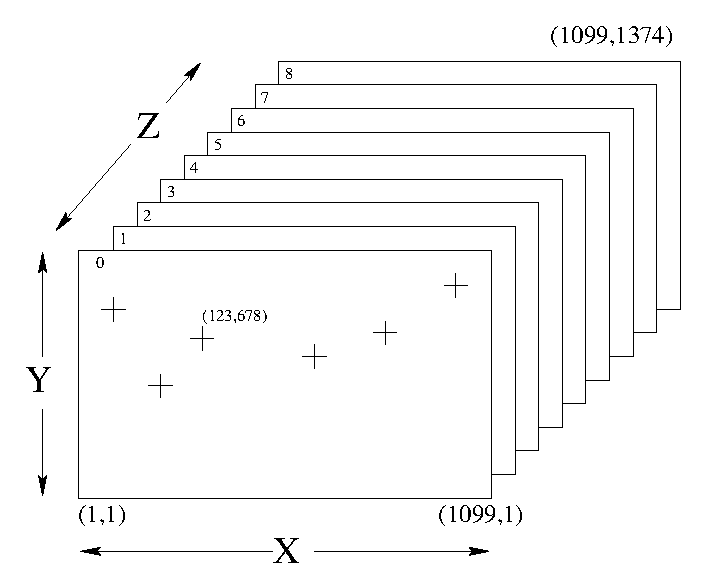
\includegraphics[width=\textwidth]{images/CubeCartoon.eps}
\caption{Cartoon of a FITS Image Cube showin the image plane in the
  intuitive sense. Using numpy to address a cube, the pixel at
  position (x=123,y=678,z=*) is addressed as cube[:,678,123] with a
  shape of (1,9). This is the reverse order of the
  cartoon.} %% \caption{{\tiny{citation}}}
\label{figure:CubeCartoon}
\end{figure}

\begin{figure}[h!]
\centering
%%\phantomsection
%%\addcontentsline{toc}{section}{}
%%\caption{} %% \caption{{\tiny{citation}}} 
%%\includepdf[angle=90,width=\textwidth]{}); %% with package pdfpages
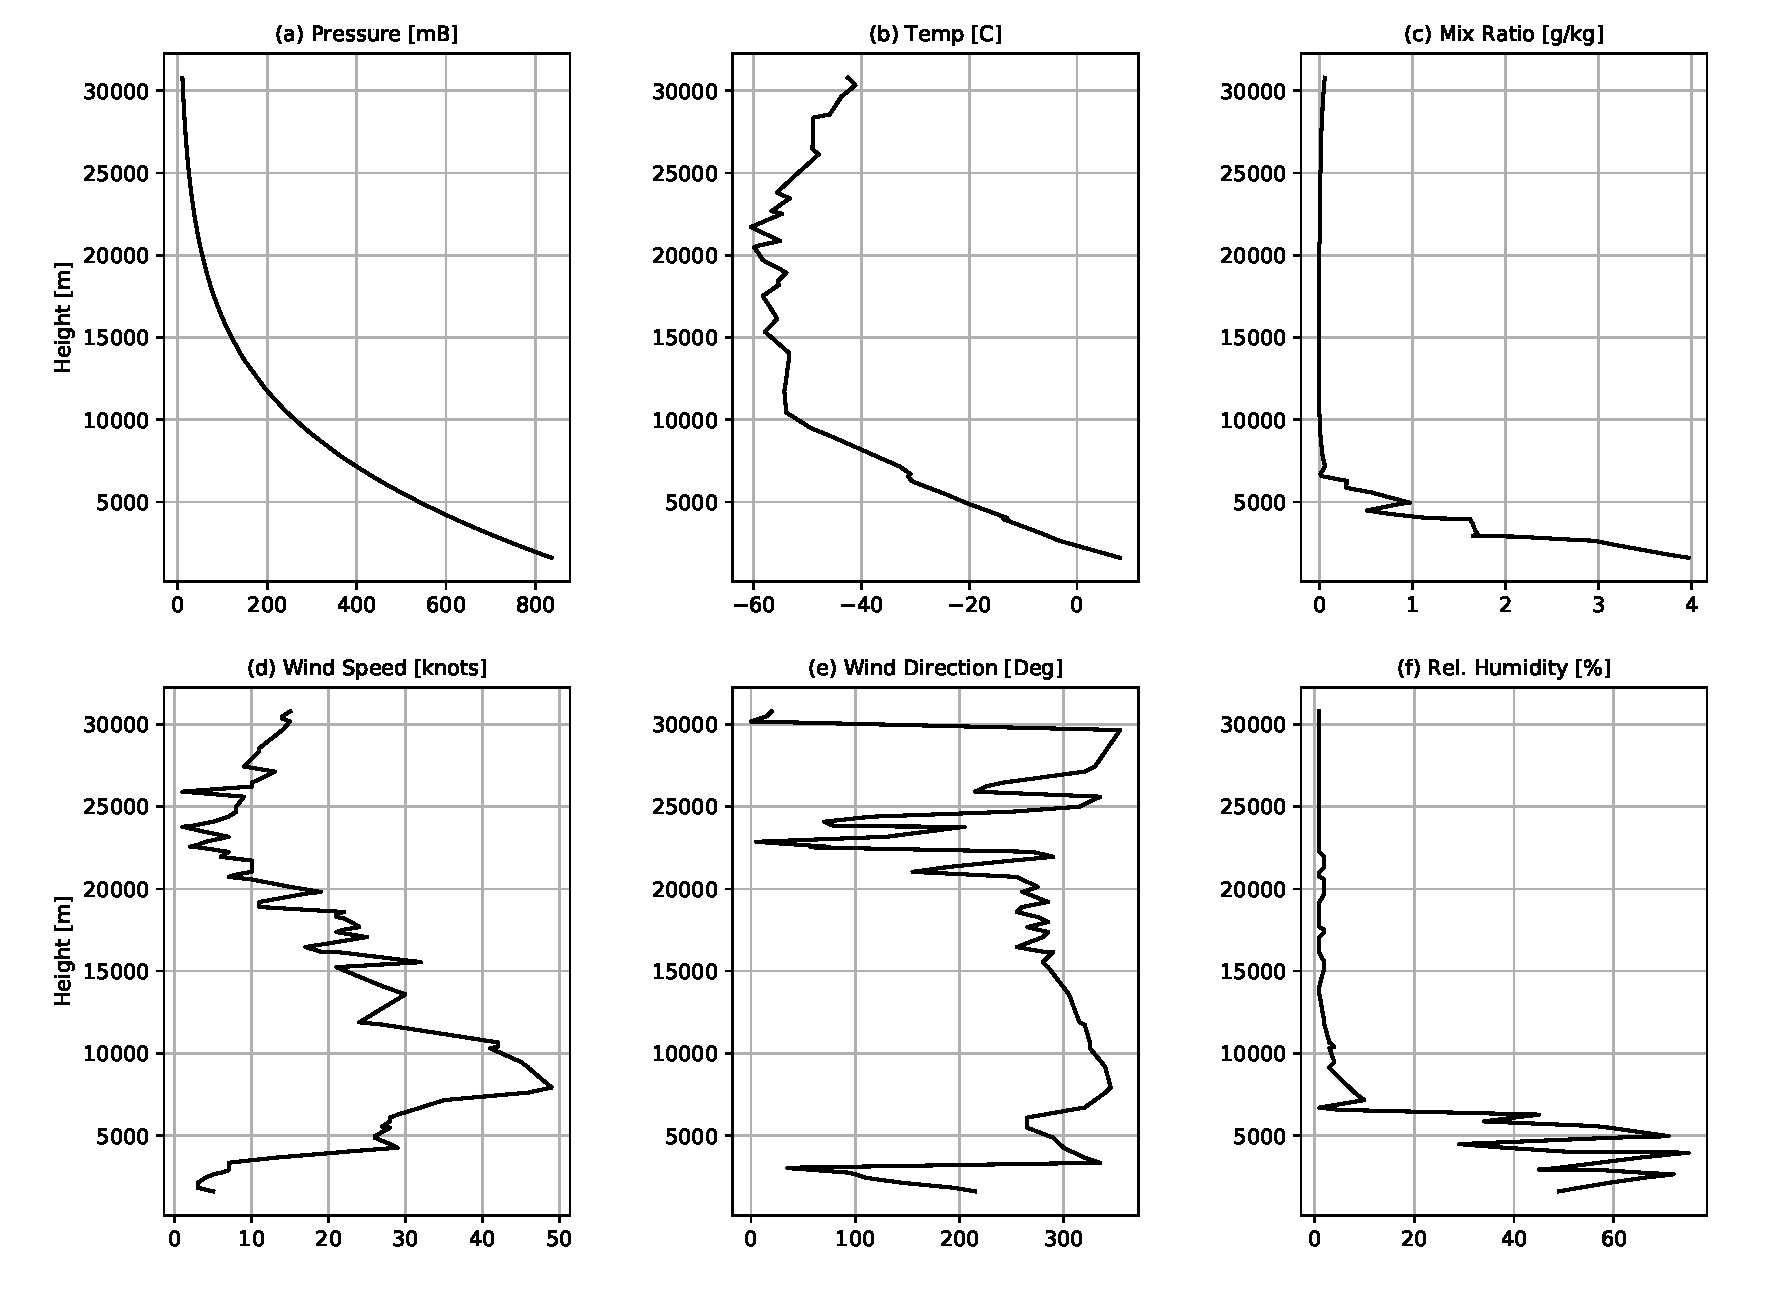
\includegraphics[width=\textwidth]{images/TypicalATM.eps}
\caption{Weather balloon data flow from Denver International Airport
  on 14 April, 2019 showing values against altitude. Note most of
  moisture is in lower atmosphere, high mixed stratospheric
  winds. ~ ~ \footnotesize{Data: University Wyoming Dept. Atm. Sciences}} %% \caption{{\tiny{citation}}}
\label{figure:WeatherPlot}
\end{figure}


%% use a bibitem approach to the references publications etc.
%% (wg-bibitem)

%%\clearpage
%%\addcontentsline{toc}{section}{References}
%%\renewcommand*{\refname}{My Bibliography and References}
%%\bibliographystyle{plain}	% bibliographystyle{apalike} and \usepackage{natbib}
%%\bibliography{MasterBib}	% expects file "MasterBib.bib"


%%\clearpage
%%\addcontentsline{toc}{section}{Index}
%%\printindex %% www.cs.usask.ca/resources/tutorials/latex/notes/toc-index.pdf

%%\begin{thebibliography}{80}
%%\usepackage{natbib}   %% bibitems
%%\end{thebibliography}

%% (wg-texdoc-endnotes)

%%%%%%%%%%%%%%%%%%%%%%%%%%%%%%%%%%%%%%%%%%%%%%%%%%%%%%%%%%%%%%%%%%%%%%%%%%%%%
% Support for endnotes
\begingroup
\renewcommand{\notesname}{Action Items}
\parindent 0pt
\parskip 2ex
\def\enotesize{\normalsize}
\theendnotes
\endgroup

\end{document}


- parallactic angle
- cosmic rays
- atmospheric effects
-- extinction
-- deflection
- optics
-- optical distortion
-- focus
-- alignment
-- slit alignment
-software
-- processing artifacts
-- sensor noise 


nrlmsise-00 C code for model atmosphere.
http://nssdc.gsfc.nasa.gov/space/model/atmos/nrlmsise00.html

Apogee 1109 images.
~/Observations/RawData/2013/nova/19Aug2013Nova
